\subsection{Selected-coordinate estimation}
\label{sec:discrete}
Physical command steps are indexed by $k$; $a_k$ denotes the supplied VLA
command and $e_k^{\rm res}$ the measured proprioceptive residual.

The calibrated FIR regression gives
\begin{equation}
z_k=f_k+w_k,\qquad
w_k=S^{-1}\!\left[\sum_{\ell=0}^{K}G_\ell(f_{k-\ell}-f_k)
 +(G_\Sigma-S)f_k+\Delta b+n_k\right].
\label{eq:main-identification}
\end{equation}
$G_\Sigma=\sum_\ell G_\ell$; $\Delta b$ is calibration bias and $n_k$ is
predictor mismatch. The history term persists for $K$ steps after a constant
fault jumps. Its bound must hold on corrected trajectories.

\begin{proposition}[Selected-coordinate target error]
\label{thm:estimator}
Let $\mathcal C$ be a coordinate box, $D$ a fixed binary diagonal mask,
$f_k,\fhat_0\in\mathcal C$, $E_k^D=\|D(\fhat_k-f_k)\|$,
$\epsilon_k^D\ge\|Dw_k\|$, and $\nu_k^D\ge\|D(f_{k+1}-f_k)\|$.
For the actual full-update flag $\chi_k\in\{0,1\}$, $0<\gamma\le1$,
and $s_k,\alpha_k\in[0,1]$, attenuation and innovation respectively satisfy
\begin{align}
E_{k+1}^D&\le(1-\chi_k\gamma)E_k^D+
\chi_k\gamma[(1-s_k)\|Df_k\|+s_k\epsilon_k^D]+\nu_k^D,
\label{eq:legacybound}\\
E_{k+1}^D&\le(1-\chi_k\alpha_k)E_k^D+
\chi_k\alpha_k\epsilon_k^D+\nu_k^D.
\label{eq:estbound}
\end{align}
\end{proposition}
Box projection is nonexpansive on the selected coordinates; a coupled convex
set need not have this property. With $D=I$, both bounds hold for any closed
convex set. The normalizer selection $P_r$ remains distinct from $D$:
uncorrected coordinates can still change $s_k$ or $\alpha_k$.
A full hold has $\chi_k=0$; target-only gating has $\chi_k=1,s_k=0$ and
retains leakage.

\paragraph{Target convergence is not pairwise contraction.}
For fixed noiseless data and attenuation $s$, the legacy map contracts toward
$\Pi_{\mathcal C}(sf)$, generally a biased target. For the scalar interior
innovation map $T(h)=h+\gamma(z-h)/[1+(z-h)^2/\rho^2]$, with
$\upsilon=(z-h)^2/\rho^2$,
\begin{equation}
T'(h)=1+\gamma\frac{\upsilon-1}{(1+\upsilon)^2},\qquad
\max_{\upsilon\ge0}T'(h)=1+\gamma/8.
\label{eq:innovation-counterexample}
\end{equation}
At $\gamma=.08,\upsilon=3$, the truth-error multiplier is $.98$ but the local
pairwise multiplier is $1.01$. Thus Eq.~\eqref{eq:estbound} does not establish
global Euclidean observer contraction.

\subsection{Applied correction and physical mismatch}
Propagate $B_k^D\ge E_k^D$ using the applicable recursion. For the snapshot
$\fhat_{\tau_k}$ used at step $k$, $0\le\tau_k\le k$,
\begin{align}
q_k&=(I-D)f_k+D(f_k-\fhat_{\tau_k})+\zeta_k,
\label{eq:main-mismatch}\\
B_k^{D,\rm app}&=\min\!\left\{
B_k^D+\sum_{j=\tau_k}^{k-1}\|D(\fhat_{j+1}-\fhat_j)\|,
\ B_{\tau_k}^D+\sum_{j=\tau_k}^{k-1}\nu_j^D\right\}.
\label{eq:applied-delay}
\end{align}
Here $\|D(\fhat_{\tau_k}-f_k)\|\le B_k^{D,\rm app}$ and
$\zeta_k$ includes native-decoder realization and command clipping.
Projection of an estimate does not ensure feasible commands.

\subsection{Scheduled execution recovery}
The following result is stated directly in execution distances, so the
certificate need not be derived from a differentiable transition. A smooth,
command-independent Riemannian metric is one sufficient construction
(Appendix~\ref{app:history-partition}). Contact and history effects must be
included in the execution state or in the stated transition remainder.
\begin{theorem}[Scheduled same-command execution tube]
\label{thm:tube}
Fix the supplied command sequence $a_k$. Let
$\xi_{k+1}^{\rm nom}=F_{\mathrm{exec},k}^0(\xi_k^{\rm nom},a_k)$ be its nominal
physical response, and let $\xi_k$ be the realized closed or reduced execution
state. Let $d_k$ be metrics on declared execution domains $\Omega_k$, chosen
independently of the supplied command and adapted estimate. Assume a declared,
time-independent physical baseline metric $\delta_{\rm phys}$ and constants
$0<c_-\le c_+<\infty$ satisfy, uniformly over $k$ and the certified domains,
\begin{equation}
c_-\delta_{\rm phys}(\xi,\xi')\le d_k(\xi,\xi')
\le c_+\delta_{\rm phys}(\xi,\xi').
\label{eq:distance-equivalence}
\end{equation}
For
$\lambda_k^{\rm exec},L_k,\eta_k\ge0$, suppose, uniformly over allowed commands
$a$ and admissible $\xi,\xi'\in\Omega_k$,
\begin{equation}
d_{k+1}\!\left(F_{\mathrm{exec},k}^0(\xi,a),
F_{\mathrm{exec},k}^0(\xi',a)\right)
\le \lambda_k^{\rm exec}d_k(\xi,\xi'),
\label{eq:sampled-contraction}
\end{equation}
and, uniformly over admissible realized and omitted states,
\begin{equation}
d_{k+1}(\xi_{k+1},F_{\mathrm{exec},k}^0(\xi_k,a_k))
\le L_k\|q_k\|+\eta_k.
\label{eq:sampled-transition}
\end{equation}
Then, for every admissible $\xi'\in\Omega_k$,
\begin{align}
&d_{k+1}(\xi_{k+1},F_{\mathrm{exec},k}^0(\xi',a_k))
\le \lambda_k^{\rm exec}d_k(\xi_k,\xi')+L_k\|q_k\|+\eta_k,
\label{eq:incremental}\\
&R_{k+1}=\lambda_k^{\rm exec}R_k+L_k\big(\|(I-D)f_k\|+B_k^{D,\rm app}+\bar\zeta_k\big)+\eta_k
\label{eq:tube}
\end{align}
bounds $X_k:=d_k(\xi_k,\xi_{k}^{\rm nom})$ from $R_0\ge X_0$ and gives
$\delta_{\rm phys}(\xi_k,\xi_k^{\rm nom})\le R_k/c_-$, provided
$\|\zeta_k\|\le\bar\zeta_k$, the supplied commands are admissible, and all
states and tubes needed to invoke Eqs.~\eqref{eq:sampled-contraction}--
\eqref{eq:sampled-transition} remain in the declared domains.
\end{theorem}
Equation~\eqref{eq:sampled-contraction} is the certificate itself and may be
verified directly for a nonsmooth sampled or hybrid transition. The Jacobian
metric inequality in Eq.~\eqref{eq:sampled-metric} is a smooth-mode sufficient
condition, not an additional theorem assumption.
This is recovery of physical execution under the same supplied commands,
not an independently rerun healthy VLA trajectory. No VLA Jacobian or
policy-state metric is needed. Arbitrary finite $\lambda_k^{\rm exec}\ge0$
give a finite-horizon bound; exponential
forgetting requires $\prod_{i=j}^{k-1}\lambda_i^{\rm exec}\le C\varrho^{k-j}$ on every
subinterval, $C\ge1$, $\varrho<1$. Hybrid events and intermediate chunk
motion must be included in the direct transition conditions. Task preservation is a separate conditional
extension (Appendix~\ref{app:task-extension}). The contraction and
transition constants were subsequently measured on the evaluated robots
rather than left open: Eq.~\eqref{eq:sampled-contraction} holds on the GR1
arm servos and fails on the Panda under operational-space control, where the
measured ratio is $1.00$ and this theorem therefore yields only its
finite-horizon form (Appendix~\ref{app:measured-certificates}). Task margins
remain uncertified.

\subsection{Closing prediction--execution coupling}
The predictor is evaluated on trajectories changed by the correction.
A trajectory-dependent residual bound therefore requires a coupled condition.
\begin{corollary}[Active-every-step recovery region]
\label{thm:discrete-region}
With $\chi_k=1$, $\tau_k=k$, suppose
\begin{equation}
X_{k+1}\le\lambda_dX_k+bE_k^D+d_0,\qquad
\|Dw_k\|\le\epsilon_0+k_EE_k^D+k_XX_k.
\label{eq:discrete-coupling}
\end{equation}
For nonnegative coefficients, let $a=1-\lambda_d>0$, $c=1-k_E>0$, $\Delta=ac-bk_X>0$ and masked drift
at most $\nu$. Set $v=\epsilon_0+\bar a_{\rm att}+\nu/\gamma$ for attenuation,
where $\bar a_{\rm att}\ge(1-s_k)\|Df_k\|$; set
$v=\epsilon_0+\nu/\underline\alpha$ for innovation with
$\alpha_k\ge\underline\alpha>0$. Any rectangle containing $(X_0,E_0^D)$,
inside the domain, and satisfying
\begin{equation}
a\bar X\ge b\bar E+d_0,\qquad c\bar E\ge k_X\bar X+v
\label{eq:discrete-rectangle}
\end{equation}
is forward invariant.
\end{corollary}
Here $b=L$ for the masked interface bound; predictor-error growth $k_X$ closes
the feedback between correction and visited states. The condition $ac>bk_X$
requires decay of the two subsystems to dominate their mutual error growth.
Appendix~\ref{app:discrete-region} gives the equality corner and a sufficient
startup budget requiring valid error and execution-domain bounds.

\subsection{An analytically verified execution instance}
For the servo in Appendix~\ref{app:contraction-example}, a constant metric
$P=\operatorname{diag}(1,4)$ satisfies $A^\top PA=.92^2P$ for the nominal
robot--controller map, giving $\lambda_k^{\rm exec}=.92$ and $L_k=2$.
It therefore verifies the smooth sufficient condition and the direct
contraction bound used by Theorem~\ref{thm:tube}.
Figure~\ref{fig:servo-main} propagates the same estimator and execution bounds
through fault onset, full-update holds, and delayed snapshots. The limiting
metric errors are $14.94$\,mm for attenuation and $5.64$\,mm for innovation,
inside bounds of $33.29$ and $9.01$\,mm, respectively.
The construction has a matched linear predictor and fixed centering bias;
it verifies the scheduled execution tube, with no trajectory-dependent
predictor mismatch or contact transition to certify. Manipulation requires
the physical closure and domain conditions stated above.

\begin{figure}[H]
\centering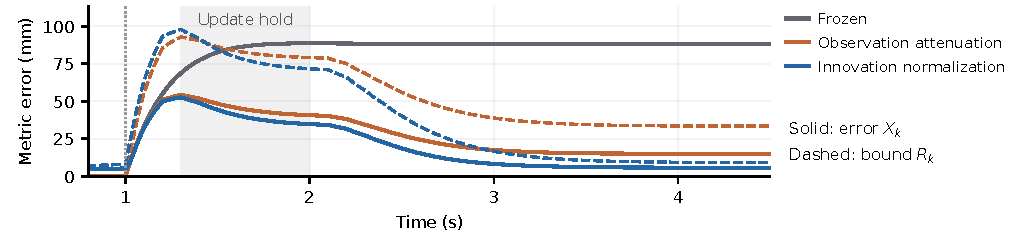
\includegraphics[width=\linewidth]{fig_servo_main.pdf}
\caption{Recovery in the analytically verified execution servo. Solid curves
show metric tracking error $X_k$; dashed curves show its propagated bound
$R_k$. The fault starts at $1$\,s; shading marks a full-update hold.
This constructed example uses the documented sampled update families and
fixed centering bias, not measured VLA trajectories
(Appendix~\ref{app:contraction-example}).}
\label{fig:servo-main}
\end{figure}
